\section{Introduction}
\label{sec:intro}

A deployed language model reads a long document. Early in the document, ``Jordan'' names a person; later, it names a country. A cache can store both observations, a nearest-neighbor memory can retrieve similar prefixes, and a test-time optimizer can move a hidden state. None of these operations fixes the structural error if the model has only one runtime concept for both cases. Every update is then forced to write incompatible consequences into the same cell. The missing object is not a better local update; it is the distinction that separates the two cells.

This paper starts from the claim that runtime learning has two fundamentally different failure modes. In a \emph{state error}, the learner is already conditioning on the right concept, but the concept's local state is stale; the right operation is repair, such as updating a cache entry, sufficient statistic, ridge solution, fast-weight memory, or local adapter. In a \emph{representation error}, the concept itself is too coarse and identifies states whose consequences differ; the right operation is refinement, namely creating a new distinction before storing the new local state. The rule is:
\begin{align*}
\textit{if the atom is wrong, refine; if the local state is wrong, repair.}
\end{align*}

\begin{figure}[t]
\centering
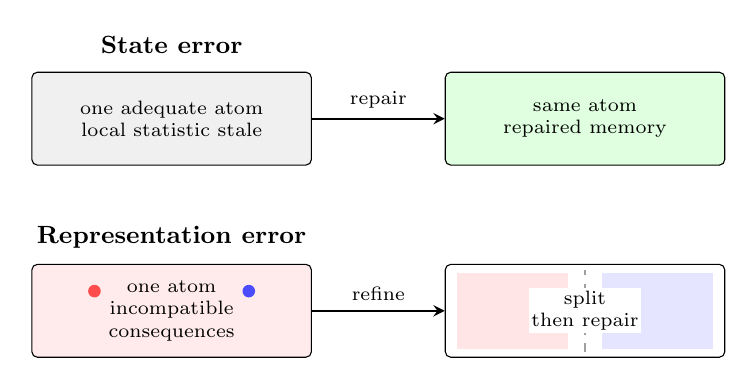
\begin{tikzpicture}[x=1cm,y=1cm,>=stealth]
\tikzset{
    panel/.style={draw,rounded corners=2pt,minimum width=3.55cm,minimum height=1.18cm,align=center,font=\scriptsize,text width=3.05cm},
    title/.style={font=\small\bfseries},
    flow/.style={->,thick}
}
\node[title] at (1.8,1.65) {State error};
\node[panel,fill=gray!12] (state0) at (1.8,0.72) {one adequate atom\\local statistic stale};
\node[panel,fill=green!12] (state1) at (7.05,0.72) {same atom\\repaired memory};
\draw[flow] (state0.east) -- node[above,font=\scriptsize] {repair} (state1.west);

\node[title] at (1.8,-0.78) {Representation error};
\node[panel,fill=red!8] (repr0) at (1.8,-1.72) {one atom\\incompatible consequences};
\fill[red!70] (0.82,-1.47) circle (0.08);
\fill[blue!70] (2.78,-1.47) circle (0.08);
\node[panel,fill=white] (repr1) at (7.05,-1.72) {};
\fill[red!10] (5.42,-2.20) rectangle (6.83,-1.24);
\fill[blue!10] (7.27,-2.20) rectangle (8.68,-1.24);
\draw[dashed,gray!75] (7.05,-2.24) -- (7.05,-1.96);
\draw[dashed,gray!75] (7.05,-1.48) -- (7.05,-1.20);
\node[font=\scriptsize,align=center,fill=white,inner sep=1pt] at (7.05,-1.72) {split\\then repair};
\draw[flow] (repr0.east) -- node[above,font=\scriptsize] {refine} (repr1.west);
\end{tikzpicture}
\caption{Runtime learning has two failure modes. Stale state should be repaired inside an adequate concept; incompatible consequences inside one atom require refinement.}
\label{fig:two-failure-modes}
\end{figure}

Many runtime-learning mechanisms implement one dominant response to surprise. Cache and $k$NN language models store or retrieve more examples \citep{grave2017improving,khandelwal2020generalization}. Fast weights and delta-rule linear attention repair associative state \citep{ba2016using,schlag2021linear}. Test-time training and adaptation optimize an inference-time surrogate \citep{sun2020test,wang2021tent,sun2025learning}. Online trees refine leaves by split scores \citep{breiman1984classification,domingos2000mining}. Sparse MoE routes to trained experts \citep{shazeer2017outrageously,fedus2022switch}. Adaptive category and prototype systems, including ART 1 and ART 2, create or move categories \citep{carpenter1987massively,carpenter1987art2,kohonen1990self,fritzke1995growing,snell2017prototypical}. DGM is not a claim that these ingredients are new. The claim is that a runtime learner should first decide which operation is legal: repair within the current information, or refine the information itself.

\begin{table}[t]
\centering
\small
\begin{tabular}{p{0.20\linewidth}p{0.31\linewidth}p{0.39\linewidth}}
\toprule
Method family & What it does when surprised & Why that is incomplete \\
\midrule
Cache/$k$NN-LM & store or retrieve more examples & does not decide whether a new concept is needed \\
Fast weights / local memories & repair associative state & cannot fix missing distinctions \\
TTT/TTA & optimize a test-time objective & treats adaptation as surrogate-loss descent \\
Online trees & split leaves & rooted hierarchy; no local repair memory at graph concepts \\
MoE / PKM & route to trained capacity & experts or keys are static, not runtime-created concepts \\
ART systems / prototypes & create or move categories & lacks edge-generated local repair structure \\
\bottomrule
\end{tabular}
\vspace{0.35em}
\begin{minipage}{0.96\linewidth}
\footnotesize
\emph{Representative references.}
Cache and $k$NN-LM: \citep{grave2017improving,khandelwal2020generalization};
fast weights and local memories: \citep{ba2016using,schlag2021linear};
TTT/TTA: \citep{sun2020test,wang2021tent,sun2025learning};
online trees: \citep{breiman1984classification,domingos2000mining};
MoE and PKM: \citep{shazeer2017outrageously,fedus2022switch,lample2019large};
ART, ART 2, and prototypes: \citep{carpenter1987massively,carpenter1987art2,kohonen1990self,fritzke1995growing,snell2017prototypical}.
\end{minipage}
\caption{Representative runtime-learning mechanisms and the single dominant update they apply when surprised. DGM's claim is not that these mechanisms are absent from prior work, but that runtime learning needs an explicit decision between refining the information structure and repairing state inside it.}
\label{tab:runtime-learning-comparison}
\end{table}

The separation is structural. A learner's information state can be represented by a partition or sigma-algebra, and its admissible predictors are precisely the measurable functions with respect to that information. If two states lie in the same atom but require different outputs, no predictor over the current information can satisfy both. More computation inside the atom cannot remove the contradiction. This is the paper's central diagnosis: a contradiction inside an atom is not a failed optimization step; it is a certificate that the atom is too coarse.

The formal core is then minimal information refinement. In a finite space, adding a binary distinction cuts exactly the old atoms crossed by that distinction and leaves all other atoms unchanged. In a general measurable space, the same operation is the join
\begin{align*}
\calF_{t+1}=\calF_t\vee\sigma(Z_t).
\end{align*}
This is the smallest information update that makes the new evidence observable, using standard language from measure-theoretic probability and statistical decision theory \citep{billingsley1995probability,kallenberg2002foundations,blackwell1953equivalent,berger1985statistical}. The value of the update is also exact: under log loss, refinement value is conditional mutual information; under squared loss, it is conditional variance reduction. Population information cannot hurt, but finite-sample estimation can. Thus a useful runtime learner should refine only when a statistically guarded gain test justifies the new distinction.

Distinction Graph Machines implement this theorem-to-algorithm path as a data structure. If contradictions require distinctions, the learner needs runtime concepts. If concepts must remain stable, each concept needs a frozen anchor. If retrieval must adapt, each concept also needs a movable centroid. If distinctions are local, the structure should add pairwise graph edges rather than rewrite a global tree. If concepts have state, each node should carry a repairable memory. A DGM therefore maintains anchored concepts, movable retrieval centroids, local memories, and distinction edges. Edges are not metadata: they are binary generators that define observable distinctions and gate future routing. When a consequence arrives, DGM either repairs local memory under fixed anchors and edges, or creates a new anchored concept and edges after a guarded refinement test.

\paragraph{Terminology.}
Throughout the paper, \emph{DGM} denotes the runtime machine as a whole. A \emph{concept} is a graph node. Each concept has a frozen \emph{anchor} $a_j$, a movable \emph{centroid} $c_j$, and a repairable \emph{memory} $M_j$. A \emph{distinction edge} is a binary generator stored between concepts. We use \emph{hard route} for the exact anchor-defined selector used in the theory, and \emph{soft read} for the differentiable edge-gated implementation. We reserve \emph{prototype} mostly for related work and for standard nearest-prototype terminology.

At one timestep, the whole mechanism has the structure in Algorithm~\ref{alg:refine-repair-template}.
\begin{algorithm}[H]
\caption{\textsc{RefineOrRepairStep} (structural template)}
\label{alg:refine-repair-template}
\begin{algorithmic}[1]
\State \textbf{Input:} runtime state and current context
\State \textbf{Read:} use the current concepts, edges, and memories to predict
\State \textbf{Observe:} receive the consequence for this context
\If{the current concept is adequate}
    \State \textbf{Repair:} update local state while keeping anchors and edges fixed
\Else
    \State \textbf{Refine:} add a concept and distinction edges, then initialize local state
\EndIf
\State \Return updated runtime state
\end{algorithmic}
\end{algorithm}
The template deliberately omits retrieval rules, edge gates, scoring buffers, and memory forms. The algorithms in Section~\ref{sec:algorithms} fill in those choices. The theory supplies the two tests behind the template: the contradiction theorem says when repair is impossible under the current information, and the value identities plus sample-split guard say when a proposed distinction is worth paying for. Thus DGM is not a generic memory with a growth heuristic; it is a runtime implementation of a decision-theoretic question: is the error measurable under the current information?

For language models, the canonical layer is DGM-Embedding. Hidden-state concepts store next-token embedding memories and produce sparse logit corrections. The read path is differentiable, so slow model parameters can learn to use DGM memory. The write path is detached and forward-only: after observing the next token, the layer repairs selected local memories or refines the concept graph without inference-time backpropagation. Projection Memory and Conservative Projection Memory (CPM) appear as local repair mechanisms once the relevant distinction structure has been fixed.

\paragraph{Contributions.}
The contribution is a separation theorem and its algorithmic realization.
\begin{itemize}
    \item \textbf{Obstruction.} We prove that some runtime errors are structurally unrepairable: if incompatible consequences lie inside one atom of the current information structure, no measurable predictor can satisfy them.
    \item \textbf{Canonical update.} We identify minimal refinement as the least information update that makes new evidence observable, and we quantify refinement value under log and squared losses.
    \item \textbf{Runtime machine.} We introduce DGM, a graph-based learner whose edges generate distinctions, whose anchors stabilize those distinctions, and whose local memories support guarded repair.
    \item \textbf{Language-model layer.} We instantiate DGM as DGM-Embedding, with differentiable sparse reads, detached forward-only writes, and an explicit bridge to projection-style repair.
\end{itemize}

\paragraph{Scope of the formal claims.}
The theorem-level question is not whether DGM is the globally optimal runtime architecture. It is: given a current information structure $\calF$, when is an error impossible to fix by any $\calF$-measurable repair, and what is the least information that must be added once a new distinction is required? Sections~\ref{sec:preliminaries}--\ref{sec:value} answer this question at the population level, and Section~\ref{sec:algorithms} gives finite-sample guarded versions for a finite candidate class. DGM and DGM-Embedding are algorithmic realizations of this refine-or-repair principle; optimization guarantees for deep nonconvex backbones and global search over all possible distinctions are outside the theorem statements.

\paragraph{Organization.}
Sections~\ref{sec:preliminaries}--\ref{sec:value} give the information-structure obstruction, the minimal refinement rule, and the value identities. Section~\ref{sec:algorithms} turns the theory into Distinction Graph Machines. Section~\ref{sec:large-model-training} gives DGM-Embedding for language models. Section~\ref{sec:technical-overview} summarizes the guarantees, Section~\ref{sec:projection-bridge} relates the repair side to Projection Memory and CPM, and Section~\ref{sec:experiments} gives computational checks.
